\section{Requirements for Android application}

\subsection{Application features}\label{FeaturesSection}

\paragraph{Vehicle Routing Problem}
Standard OptaPlanner distribution \cite{OptaPlannerDistribution} contains demonstration examples. One of the examples is
Vehicle Routing application. Its source code already contains Vehicle Routing Problem model which should be included in
this application. Also it contains some tools for importing specific \texttt{.vrp} files. Graphical user interface
cannot be ported because application is written by Awt and Swing libraries which are not included in Android API as
described in Section \ref{OptaPlannerChapter}. Thanks to that and because it is good practise to adapt the application
to Android mobile platform, graphical user interface and functions of application should be completely rewritten and
adjusted to fulfill aspects of Android application development.

\paragraph{Application settings}
Application without any settings is too static and user cannot do much with it. Therefore, it should be option to choose
problem solving algorithm which can show that not all algorithms are suitable for such problems. Another option should
be setting of the time limit of caculation. Thanks to this, when process is terminated, last solution should remains
shown on the screen. It should be also possible to terminate process before time limit manually.

\paragraph{File opening}
Original Vehicle Routing application contains \texttt{.vrp} example files. These files should be compatible with created
application and some of them should be included. It should be possible to open these files and display them similar way
as in original application.

\paragraph{Solution diplaying}
When user selects file, unsolved solution should be displayable on the application screen. After start of solving
process, new best solution also should be displayable every time when new it is found. Application should further
contains resources how to display actual statistic information about solved problem.

\paragraph{License}
Whole application should be distributed as opensource software and it should be written under Apache License 2.0.
Source code must be publicly available on the internet to guide other persons how to use OptaPlaner in their projects.

\subsection{Android devices support}
Before the development starts, it is good to clarify for which version of Android will be application supported. Every
version of Android comes with new API and new functionality. Biggest changes comes when first number of version is
changed. Table \ref{distributon} shows actual distributions of Android verisons on devices.

Versions 2.x.x are on the decline, the most used versions are 4.x with higest percentage representation and the newest
version 5.x is not so much used yet but their participation grows. Therefore it was decided that application should
supports android from version 4.0 (API 14). It desides which resource can be used for application proposal and
development and how application should be tested.

\begin {table}[h!]
    \begin{tabular}{|c|c|r|}
        \hline
        Android version   & API   & Distribution  \\ \hline \hline
        2.2               & 8     & 0.4 \%        \\ \hline
        2.3.3 -- 2.3.7    & 10    & 6.4 \%        \\ \hline
        4.0.3 -- 4.0.4    & 15    & 5.7 \%        \\ \hline
        4.1               & 16    & 16.5 \%       \\ \hline
        4.2               & 17    & 18.6 \%       \\ \hline
        4.3               & 18    & 5.6 \%        \\ \hline
        4.4               & 19    & 41.4 \%       \\ \hline
        5.0               & 21    & 5.0 \%        \\ \hline
        5.1               & 22    & 0.4 \%        \\ \hline
    \end{tabular}
    \centering
    \caption{Android version distributon \cite{Dashboards}}
    \label{distributon}
\end{table}

\section{Application proposal}

\subsection{Application features}

\paragraph{Application settings}
Application will supports several settings options. It is possible to select one of three algorithms: First fit
decreasion with late acceptance, branch and bound and brute force. Simultaneously, it is required to select time limit
of calculation in seconds. Calculation stops after time limit is reached or it is possible to stop it earlier by play
button. Another settings option is selection of solved example. Application contains list of files and after user select
one of them everything will be prepared to calcultion start. These setting will be diplayed on the first screen of
the application.

\paragraph{Vrp files}
Mentioned list of example files will consist from files used in original OptaPlanner application. These files are named
same way so user can compare results between both applications. Because Android system by default does not contain file
browser and user probably do not have own \texttt{.vrp} files, application will not support opening files from device
storage. List of files will be placed on the second screen of the application.

\paragraph{Porting of Vehicle Routing Problem model}
In Section \ref{FeaturesSection}, it was decribed that original application already contains Vehicle Routing model for
OptaPlanner tool. These classes will be used and embedded into application and will be used to calculation of the
problem. Further, it will be useful to displaying current solution.

\paragraph{Problem solving}
Graphical user interface cannot wait until calculation is finished and therefor these two parts must be separated from
each other. While solving is in progress, user will control the application and use some of its parts. Typical problems
with Android application will be solved. When screen is turned or application is hidden in background, solving process
have to be still active and not to be stopped. Solution will be displayed as desribed bellow.

\paragraph{Solution displaying}
New best solution will be displayed every time when it is found. For that purpose application will contain third screen
specially for this displaying. Solution will be similar to original application. Lines will present roads, vehicles and
depots will have own icon. Customers will be different because saving screen space. Intead of point with number it will
be presented as circles with inner number describing its demand. Time window problem will be displayed in a similar way
but not separated from customer.

\paragraph{Solution data}
Every solution has data which cannot be displayed graphically or they are so important that should be displayed
separately. From that reason, score of solution and actual load of vehicles will be drawn on side menu which will be
described bellow.

\subsection{Design of screens}

\paragraph{Application top bar}
Top bar will be placed on the top of the each screen. It will contain name of the application and quick functions
buttons. These buttons can start the calculation or call the informational dialogs. Buttons do not have to be visible
all the time but only on the screens when it necessary.

\paragraph{Settings screen}
This screen will be main screen of the application. It consists of top bar welcome text and settings part where
calculation options can be set. Last element on the screen is button for switch to next screen where vrp file can be
selected.

\paragraph{Screen with vrp files list}
Whole screen constains only list of vrp files and top bar. Top bar on this screen does not contain any buttons because
no ones are needed here. List contains all included vrp files in application. After click on one of them screen will be
switched to the last solution screen.

\paragraph{Screen of solution}
More important screen of application will be solution screen. Solution and its gradual progress is displayed on this
screen. On the top bar, button for start of calculation will be included. Under the actual solution representation,
progress bar for displaying actual time will be placed. When user swipe with finger from left to right on the screen,
side menu with actual solution statistic will be displayed.

\paragraph{Side menu with statistics}
This menu is displayed on right side on the solution screen. It contains data statistic of actual solution. First item
of menu is solution score and next items represent every vehicle in the solution and its current load and capacity.
Menu can be close when user clicks somewhere outside menu.

\begin{figure}[h!]
    \centering
    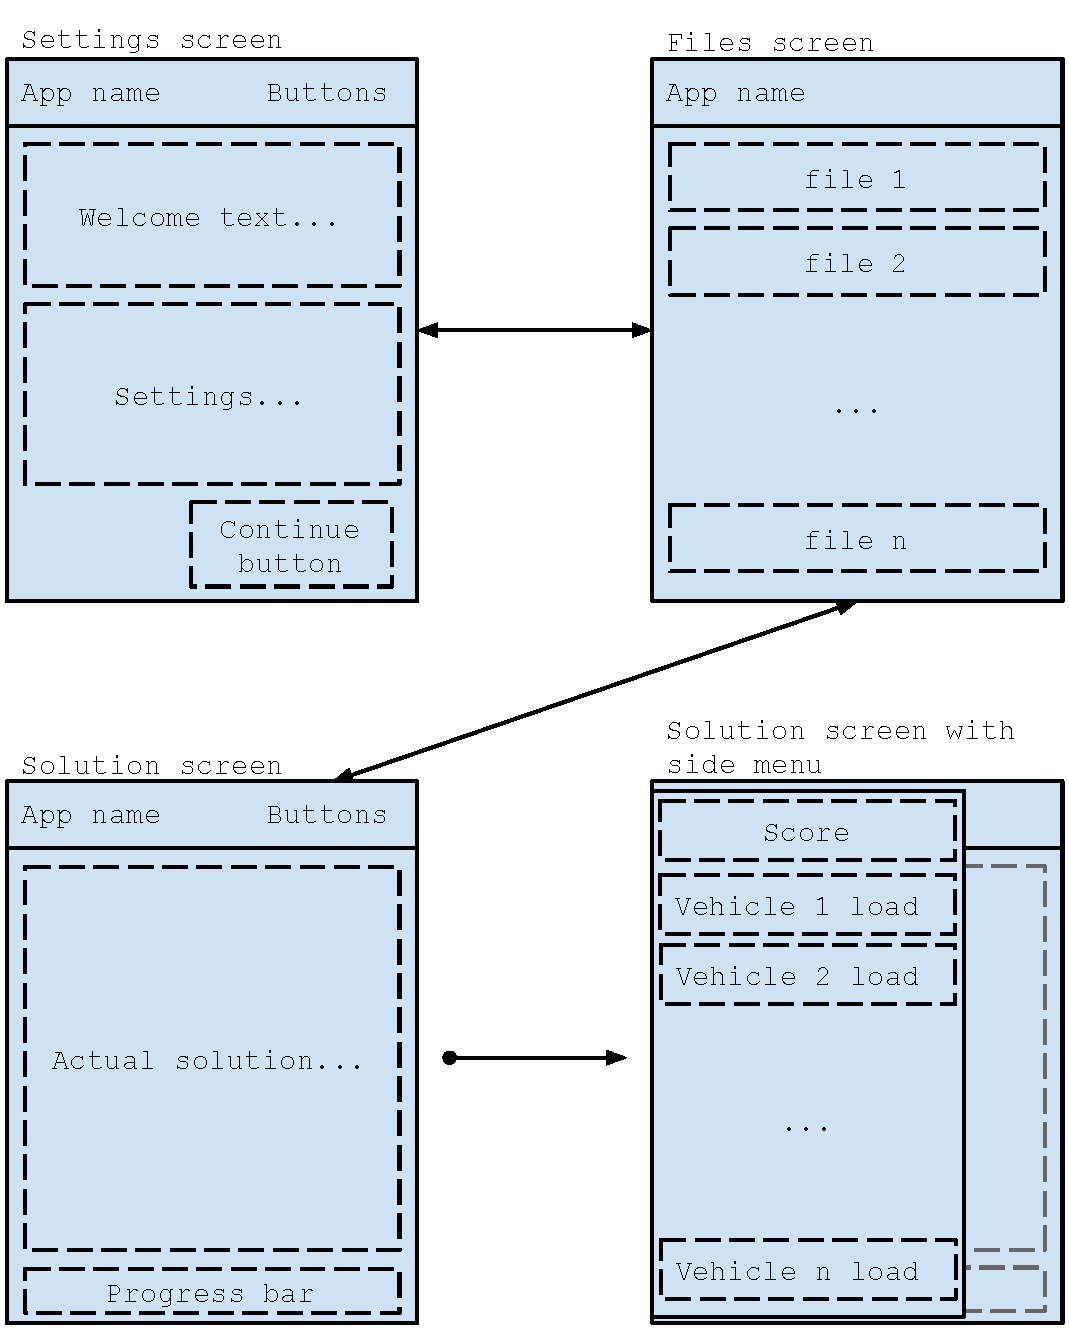
\includegraphics[scale=0.8]{fig/proposal.pdf}
    \caption{Proposal of screens}
    \label{proposalFig}
\end{figure}

\paragraph{Informational dialogs}
Application will contains two informational dialogs to better understanding application content. First one will contain
information about application itself. Second one will consist from legend which describes all displayed components of
Vehicle routing problem on the screen.

\paragraph{Material design}
One of the new features which bring Android version 5 is material design. It is very sophisticated study that show how
to handle with with elements, layouts, colors and more. Although this property is not fully backward compatible, it is
possible partially to bring this design to earlier devices with older versions of Android. This application uses
material design as much as possible. Every screen will contains material design elements which are described bellow.
